\begin{displayquote}
	\textsf{Different optimization techniques for Krylov iterative methods were developed to accelerate convergence during linear system solving to reduce the number of iterations and to calculate solutions in the shortest possible time. UCGLE and $m$-UCGLE are more complex since it is the combination of several different computational components. Thus a large number of parameters have impacts on its numerical and parallel performance. The purpose of this chapter is to design adaptive methods to automatically optimize and select these parameters so that they can be adapted to different systems and hardware. In this chapter, we will at first study different autotuning schemes and optimizations that have contributed to it. Then we will focus on the propostion of heuristic to automatic selection of Least Squares Polynomial degree of UCGLE at runtime.}
\end{displayquote}

\vspace{0.6in}

\section{Autotuning}

Current supercomputer architectures have complex architecutures, with milions of cores utilizing non-uniform memory access and hierarchical cases. The introduction of GPUs and other accelerate increases the heterogeneity of computers. Thus, tuning the performance of softwares is increasingly become difficult. Moveover, the science and industrial applications on the supercomputing systems tends to be more and more complex. It is necessary to propose strategies and methologies to autotune them for achieving the best performance. Autotuning refers to the automatic generation of a search space of possible implementations of a computation that are evaluated through models and/or empirical measurement to identify the most desirable implementation \cite{balaprakash2018autotuning}. The main goal of autotuning is the minimization of execution time of applications. If the autotuning schemes with different objectives are combined together, this might achieve to optimize the parallel performance, the energy efficiency and reliability of applications.

In the first part of this section, we present several types of optimizations that are relatively different in appearance, but with the same goal: the reduction of the calculation time to arrive at solution.


\subsection{Different Levels  of Autotuning}

Different aspects influence the performance of applications on supercomputers. In this section, we discuss the different levels of autotuning. 

	\subsubsection{Algorithm autotuning}
	
	For a fixed application, different numerical methods are available to solve this problem. Numerical toolkits such as PETSc and Trilinos provide a large number of parallel solution methods for large sparse linear systems and eigenvalue problems, including the direct solvers and iterative solvers with different preconditioning techniques. It is difficult for the user to select the routines to correctly and efficiently solve the problems. Lighthouse Project \cite{norris2014lighthouse} classified the solvers and preconditioners based on a small number of features of problems using the machine learning methods. These classifiers are trained based on a large number of training set of linear systems and eigenvalue problem. For the practioner, the features of systems are used as the input, and the output is a collection of solver and their configurations that are probable to perform well. In \cite{nair2014generating}, Nair et al. describes the development of this approach with a focus on the analysis of sparse egiensolvers provided by SLEPc.
	
	\subsubsection{Code variant autotuning}
	
	Code variants may affect code organization, data structures, high-level algorithms, and low-level implementation details. In detais, code variants in complex applications represent alternative implementations of a computationl operation. For each code vriant, it has the same interface, and is functionality equivalent to the other variants but may employ fundamentally different algorithms or implementations strategies \cite{muralidharan2016architecture}. A well-known example is the implementation of SpMV operation, which is the kernel of Arnoldi reduction of Krylov iterative methods. In Tpetra package of Trilinos, the SpMV operation is implemented with different matrix storage format (CSR or Row matrix) with different strategies across different parallel arcitectures, e.g. MPI for distributed-memory systems, OpenMP and POSIX Threads for shared memory platforms, and CUDA for GPUs. \cite{aquilanti2011parallel}, Aquilanti et al. proposed the autotuning strategy for the incomplete orthogonalization inside parallel GMRES. Different Domain Specific Languages and code generation strategies are also provided, which are able to generate the parallel optimized code variant specified for different computing architectures from a serial algoritms, e.g., PATUS \cite{christen2011patus} presented by Christen et al., which is a code generation and autotuning framework for parallel iterative stencil computations on modern microarchitectures; and Pochoir \cite{tang2011pochoir} a DSL language in which the user only specifies a stencil (computation kernel and access pattern), boundary conditions and a space-time domain while all optimizations are handled by a compiler.
	
	In \cite{demmel2005self}, Demmel et al. described the approaches for obtaining tuned high-performance kenerls and for automatically choosing suitable algorithms. ATLAS (Automatically Tuned Linear Algebra Software (ATLAS)) \cite{whaley1998automatically} is a library optimized for the analysis of dense problems, and PHiPAC (Portable High Performance ANSI C) \cite{bilmes1997optimizing} is a library designed with similar purposes but for sparse problems. OSKI (Optimized Sparse Kernel Interface) library implemented by Vuduc et al. \cite{vuduc2005oski} is a collection of low-level primitives that provide automatically tuned computational kernels on sparse matrices, for use by solver libraries and applications. A fully run-time auto-tuned sparse iterative solver with OpenATLib was introduced by  Naono et al. \cite{naono2012fully}. OpenATLib is carefully designed to establish the reusability of AT functions for sparse iterative solvers. Using APIs of OpenATLib, a fully auto-tuned sparse iterative solver called Xabclib was developed, which has several novel runtime AT functions.  Xabclib provides numerical computation policy that can optimize memory space and computational accuracy.
	
	\subsubsection{Hardware autotuning}
	
	In order to achieve performance portability, decisions on parallelization (how much an how many levels of parallelism) and memory hierarchy optimizations (e.g., data placement, blocking/tiling and tile size) will necessarily depend on the architecture, e.g. Chen et al. \cite{chen2007model} proposed a model-guided empirical optimization for memory hierarchy;  Ren at al. \cite{ren2008tuning} introduced a tuning framework for software-managed memory hierarchies, and Katagiri et al. \cite{katagiri2012smart} presented a smart tuning strategy for restart frequency of GMRES(m) with hierarchical cache sizes.
	
	\subsubsection{Parameter autotuning}
	
	The modern applications on supercomputers are complex. Both their numerical and parallel performance depends on different parameters, e.g., for the Krylov iterative methods with restart strategy, if the Krylov subspace size $m$ is small, their parallel performance is good, since the reduction of the requirement of  memory and SpMV operations, but small $m$ might slow down even diverge the iterative methods for solving selected linear systems, which results in the increase of time and energy consumptions. Thus for the parameter $m$, an autotuning strategy should be proposed to make a balance between its numerical and parallel performance.

\subsection{Selection Modes}

The autotuning for the code variants and parameters can be constructed according to different modes. In this section, we discuss the empirical search, the machine learning based and the automatic contectual selection.
	
\subsubsection{Empirical Search Selection}

The simplest approach for the selections is to execute each code variant, measure its runtime (or other objective function), evaluate the performance of all variants, select the best one, and include that variant in the final code to be run. These are called empirical autotuners. For a compute kernel of a sparse matrix, the implementation space is the set of data structures and implementations corresponding to these structures. Each structure is designed to improve the locality (thus improving computational performance) by exploiting a class of hollow format with specific characteristics: blocks, diagonals, bands, symmetry or the combination of all this. Structural evaluation can only be done at runtime, because knowledge of certain information will only be possible at this stage, for example, the format of the matrix makes it possible to deduce the necessary transformations in order to optimize performance. Thus, the analysis is based on heuristic and empirical data taking into account not only the data used at runtime, but also the mathematical context, for example calculating the eigenvalues of matrix using Krylov method may require to transform the matrix from one to another. Such a permutation (ranks and columns) can favorably alter the structure of A by improving the locality of its elements, without changing the eigenvalues. But, this type of analysis can only take place at runtime. Indeed, while in this context the study focuses negligible compared to the gains obtained, an analysis out of context execution is much too prohibitive to be exploited in practice (apart from a few exceptions).


\subsubsection{Machine Learning Based Selection}

Because the search space may be large, intelligent search methods and models may be used to iteratively prune the variant space as evaluation takes place. Instead of executing trials directly, some autotuners may train models from trial executions or from historical data. A runtime prediction model can be used as a proxy for real kernel executions, which allows a tool to more rapidly search the tuning parameter space, especially for long-running kernels. Models arising from training are particularly useful when selection depends on input data or other aspects of execution context; such decision models are consulted at runtime to select variants based on contextual features. Application developers may also embed hints in their code to influence the choice of variant at runtime.

When analytical performance models become too restrictive for a given scientific workload and HPC architecture, empirical performance modeling is an effective alternative. In this approach, a small subset of parameter configurations (code variants) is evaluated on the target machine to measure the required performance metrics, and a predictive model is built by using machine learning approaches. Here, the choice of the supervised machine learning algorithm for building the surrogate performance model is crucial. Often this choice is driven by an exploratory analysis of the relationship between the parameter configurations and their corresponding runtimes. A typical model-based approach is a two-step process in which an analytical or empirical model is built first and a search algorithm is used to find high-performing configurations using the model.

In recent years, a new class of empirical model-based search has received considerable attention and has been shown to be effective for autotuning. This approach consists of sampling a small number of input parameter configurations and progressively fitting a surrogate model over the input–output space until exhausting the userdefined maximum number of evaluations. The surrogate model is iteratively refined in the promising input parameter region by obtaining new output metrics at input configurations that are predicted to be high performing by the model. Bergstra et al. \cite{bergstra2012machine} presented a method for predictive auto-tuning based on boosted regression trees. They showed that machine learning methods for non-linear regression can be used to estimate timing models from data, capturing the best of both approaches. Nitro \cite{muralidharan2014nitro} is a framework for adaptive code variant tuning, which  provides a library interface that permits programmers to express code variants along with metainformation that aids the system in selecting among the set of variants at runtime. Machine learning is employed to build a model through training on this meta-information, so that when a new input is presented, Nitro can consult the model to select the appropriate variant. Falch et al. \cite{falch2015machine} presented a machine learning based auto-tuning for enhanced opencl performance portability. MasiF introduced by Collions et al. \cite{collins2013masif} is a tool to auto-tune the parallelization parameters of skeleton parallel programs. It reduces the size of the parameter space using a combination of machine learning, via nearest neighbor classification, and linear dimensionality reduction using PCA.

\subsubsection{Automatic Contextual Selection}

The role of the analysis and dynamic adaptation of the algorithm is to adapt certain parameters of the iterative methods in order to accelerate their due convergence of the method and / or that of preconditioning. These techniques are used at runtime and depend on heuristics computed at this time without dependence on the data or on the computing environment (whether software or hardware). Also, interactions on the part of the user can be useful to assist and optimize autotuning. In addition, these techniques also have the role of assisting the user during the parameterization by proposing tuners for a specific purpose (minimizing the calculation time, maximizing numerical accuracy, etc.). All of this will be explored in the following sections through the autotuning of the GMRES subspace size (m) and the truncation parameter of the Arnoldi orthogonalization process.

The approach that we have just presented is focused on the contextual optimization of the computation, be it material or structural, other optimization techniques exist, some rely on a selection of numerical methods, it is is that we go now.

\iffalse
\subsection{Autotuning Techniques For Numerical Methods}

The contextual optimization of the computation is an approach of selection of software bricks in order to extract the maximum of performances of a material and mathematical context to solve a given problem, in this case to solve a system of equations linear through an iterative method of Krylov.

\begin{enumerate}

\item\textbf{Material evaluation}

The idea is to analyze, in several steps, via benchmarks and automatically, the performance of software bricks for a given hardware platform (parallel, for example, a cluster or a computing grid) and to determine a set prerequisite for optimizations [21]. These software bricks are, in a non-exhaustive way, the type of storage of the matrix (CSR, CSC, Ellpack, and block variants) [55], the size of the blocks if an appropriate storage format is used [56], the type of product matrix vector [35], the loops depth of loops, the software pipelining strategies, the allocation of the registers and the ordered loops of the iterative methods used (especially for the orthogonalization method, we will think of Gram-Schmidt). The choice of these software building blocks thus relying, as we have mentioned, on benchmarks and on intrinsic considerations to the hardware (size of the different levels of caches, latency between the memories and the number of nodes of the cluster or the grid ), the evaluation is performed by executing each implementation on synthetic matrices, only once. This makes it possible to characterize the material context independently of the problem that will be treated [83].


In the case of sparse matrices, these optimizations are interesting to implement because of the dispersion of the values the imposing components of choosing a suitable format almost for each case or type of application. This is for example the case of the locality of the data on the hierarchy of memories (registers, levels of cache memory, random access memory, disk memory) and their distribution on the various nodes of the cluster (one will focus on the cluster, but our study also applies to grids). Moreover, their size being, in general, rather important it is advisable to choose a storage taking into account this sparse structure while preserving the memory.

Taking into account the hierarchy of the memories is important, because the latency to access a data in RAM is much greater than in the case where this data was present in cache whatever the level, it is therefore necessary to define a format that minimizes local latency to access the various elements of the matrix, allows the reduction of the number of communication by maximizing the number of data exchanged in order to cover the time devolved to them by calculation. This is even more true when we consider the distribution of a hollow matrix on the different nodes of a cluster, in this case it is necessary to reduce as much as possible the communications, the latency to access a data being even more important [ 24, 55, 56].
We have just established the importance of storage in relation to the hollow structure of the matrices, but this without taking into account the arithmetic operations to be carried out in the case of iterative methods. The recurrent operations are the vector vector product, the vector scalar product and the most important, the vector matrix product. The latter is central to the Krylov methods, hence the importance of the data locality in order to obtain maximum performance of the hardware platform [23, 85]. In this case, the type of storage is taken into account, but also the concept of pre-fetching the data to minimize the latency during this type of operation. These constraints will be respected, but this without presuming optimizations specific to the algorithmic of the iterative methods. For this case, depending on the method and its implementation, we can consider a reordering of loops such as inner and outer product.

From the contextual optimization of the computation we have only addressed the material-specific part, recalled the benchmarks and the selection criteria, also mentioning the fact that the process was carried out in several stages. We have highlighted the first (the selection with respect to the hardware context of execution) allowing to create sets of optimizations. These sets of optimizations make it possible to characterize the machine independently of the matrices that will be used to solve linear system resolution problems via iterative methods. As soon as the sparse is known during execution, the perfomances are then estimated according the structural properties of the matrix.

These heuristic models combining the benchmarks and the matrix-specific data make it possible to predict the structure with the most efficient performance in terms of performance, what will be called the structural evaluation.

\end{enumerate}


\textbf{Krylov Subspace Size}: Autotuning of times and convergence together.

\begin{algorithm}[htbp]{}
	\caption{Autotuning Krylov subspace size of GMRES}   
	\label{alg:gmres-krylov-autotuning}   
	\begin{algorithmic}[1]
		
		\Function {Auto-Subspace}{$input$: $m_{min}$, $m_{max}$}
		\State $i=1$
		\State $m_i=m$
		\While{not converged}
		\If{$cr > cr_{max}$ or $i = 0$}
		\State $m_i=m_{max}$
		\ElsIf{$cr < cr_{min}$}
		\If{$m_{i-1} -d \geq m_{min}$}
		\State $m_i = m_{i-1}-d$
		\Else
		\State $m_i=m_{max}$
		\EndIf
		\EndIf
		\State GMRES($m_i$)
		\State $i=i+1$
		\State $cr \leftarrow \frac{||r_i||_2}{||r_{i-1}||_2}$
		\EndWhile
		\EndFunction
	\end{algorithmic}  
\end{algorithm}
\fi


\section{Automatic Selection of Least Squares Polynomial degree at runtime}

\subsection{Parameter evaluation}

\begin{enumerate}
	\item BGMRES Component
	\begin{enumerate}
		\item $m_g$: BGMRES Krylov Subspace size
		\item $\epsilon_g$: relative tolerance for BGMRES convergence test
		\item $P_g$: number of computing units for each BGMRES
		\item $l$: number of times that polynomial applied on the residual before taking account into the new eigenvalues
		\item $L$: number of BGMRES restarts between two times of B-LSP preconditioning
		\item $s$: number of RHSs
	\end{enumerate}
	\item $s$-KS Component
	\begin{enumerate}
		\item $m_a$: $s$-KS Krylov subspace size
		\item $r$: number of eigenvalues required
		\item $\epsilon_a$: tolerance for the $s$-KS convergence test
		\item $P_a$: number of computing units for $s$-KS
		\item  $\sigma$: shifted value
	\end{enumerate}
	\item B-LSP Component
	\begin{enumerate}
		\item $d$: Polynomial degree of B-LSP
	\end{enumerate}
\end{enumerate}

\subsection{Criteria}

\begin{figure}[htbp]
	\centering
	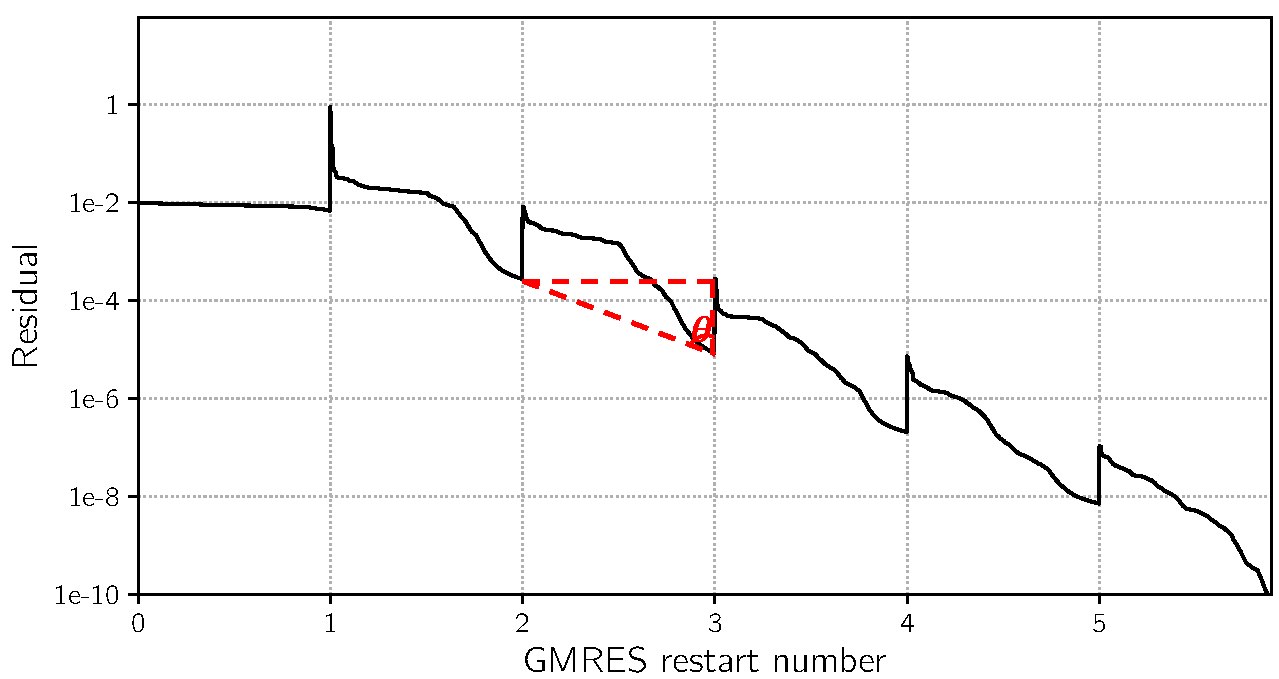
\includegraphics[width=0.99\linewidth]{fig/convergence_tuning.pdf}
	\caption{GCR-DO workflow.}
	\label{fig:cos}
\end{figure}

\begin{equation}
cr_i=\cos\angle(r_i,r_{i-1})=\frac{||r_i||_2}{||r_{i-1}||_2}
\end{equation}


\begin{equation}
t_i=\frac{t}{m_g}
\end{equation}

\subsection{Heuristic}

\subsection{Evaluation}

\section{Conlusion}

\clearemptydoublepage